\documentclass[conference]{IEEEtran}
\IEEEoverridecommandlockouts
\usepackage{cite}
\usepackage{tabularx}
\usepackage{amsmath,amssymb,amsfonts}
\usepackage{graphicx}
\usepackage{textcomp}
\usepackage{xcolor}
\usepackage{url}
\usepackage{caption}
\usepackage{pgfplots}
\pgfplotsset{compat=1.18}

\def\BibTeX{{\rm B\kern-.05em{\sc i\kern-.025em b}\kern-.08em
    T\kern-.1667em\lower.7ex\hbox{E}\kern-.125emX}}
\begin{document}

\title{\textbf{Metode \textit{Gauss-Legendre} untuk Penyelesaian Integral Tentu Secara Numerik}}

\author{
\IEEEauthorblockN{Bonifasius Raditya Pandu Hendrianto}
\IEEEauthorblockA{\textit{Teknik Komputer (2306242350)} \\
\textit{Universitas Indonesia}\\
Depok, Indonesia \\
radityahendrianto@gmail.com}
}

\maketitle

\begin{abstract}
Integrasi numerik merupakan alat esensial dalam sains dan rekayasa untuk menyelesaikan integral yang sulit atau tidak mungkin diselesaikan secara analitik. Studi ini berfokus pada penyelesaian integral tentu $\int_{-3}^{3} \frac{1}{1+x^2} dx$ dengan menggunakan salah satu metode kuadratur yang paling efisien, yaitu formula Gauss-Legendre. Penelitian ini bertujuan untuk menerapkan formula Gauss-Legendre dengan dua hingga enam titik untuk mengaproksimasi nilai integral tersebut. Hasil dari setiap formula akan dibandingkan dengan solusi analitik eksak untuk menganalisis akurasi dan tingkat konvergensi metode. Analisis ini akan menunjukkan bagaimana penambahan jumlah titik dalam formula secara signifikan meningkatkan ketepatan hasil aproksimasi.
\end{abstract}

\begin{IEEEkeywords}
KEYWORD: \\
integrasi numerik, formula Gauss-Legendre, kuadratur Gauss, galat relatif, aproksimasi integral
\end{IEEEkeywords}

\section{PENDAHULUAN}

Dalam kalkulus, integral tentu merupakan konsep fundamental untuk menghitung luas di bawah kurva. Meskipun banyak fungsi dapat diintegrasikan secara analitik menggunakan teorema dasar kalkulus, terdapat banyak kasus di mana fungsi (integrand) terlalu kompleks atau hanya diketahui pada titik-titik diskrit, sehingga solusi analitik tidak dapat diperoleh. Untuk mengatasi masalah ini, metode numerik menawarkan pendekatan alternatif untuk mengaproksimasi nilai integral.

Salah satu metode integrasi numerik yang paling kuat adalah Kuadratur Gauss, khususnya formula Gauss-Legendre. Metode ini lebih unggul dibandingkan metode lain seperti Aturan Trapesium atau Simpson karena mampu mencapai akurasi yang lebih tinggi dengan jumlah evaluasi fungsi yang lebih sedikit. Keunggulannya terletak pada pemilihan titik-titik evaluasi (abses) dan bobotnya secara optimal.

Tujuan utama dari penelitian ini adalah untuk mendemonstrasikan aplikasi formula Gauss-Legendre dua-titik hingga enam-titik untuk menyelesaikan integral tentu $\int_{-3}^{3} \frac{1}{1+x^2} dx$. Hasil dari setiap aproksimasi akan dihitung dan dibandingkan dengan nilai eksak dari integral tersebut untuk menghitung galat relatif sejati ($\epsilon_t$). Analisis ini akan mengilustrasikan efisiensi dan konvergensi dari metode Gauss-Legendre seiring dengan bertambahnya jumlah titik yang digunakan.

\section{STUDI LITERATUR}

Perhitungan integral merupakan salah satu pilar utama dalam kalkulus dan rekayasa, digunakan untuk menentukan kuantitas total dari suatu laju perubahan, seperti luas, volume, atau perpindahan. Secara umum, terdapat dua pendekatan fundamental untuk menyelesaikan integral tentu: pendekatan analitik dan pendekatan numerik.

\subsection{Integrasi Analitik: Pencarian Solusi Eksak}
Integrasi analitik, atau yang sering disebut integrasi simbolik, adalah metode yang didasarkan pada Teorema Dasar Kalkulus. Pendekatan ini bertujuan untuk menemukan fungsi antiturunan (antiderivative) dari fungsi yang diberikan (integrand). Jika $F(x)$ adalah antiturunan dari $f(x)$, maka integral tentu dari $f(x)$ dari $a$ ke $b$ dapat dihitung secara eksak sebagai:
\begin{equation}
    \int_{a}^{b} f(x) \,dx = F(b) - F(a)
\end{equation}
Hasil dari metode ini adalah solusi yang pasti benar (eksak) dan bebas dari galat aproksimasi. Namun, kelemahan utamanya adalah banyak fungsi, terutama yang muncul dalam permasalahan rekayasa kompleks, tidak memiliki antiturunan dalam bentuk fungsi elementer. Contoh klasik adalah fungsi Gaussian, $\int e^{-x^2} dx$, yang tidak dapat diselesaikan secara analitik. Keterbatasan inilah yang mendorong pengembangan metode numerik.

\subsection{Integrasi Numerik: Pendekatan Aproksimasi}
Ketika solusi analitik tidak dapat ditemukan, integrasi numerik menawarkan alternatif yang kuat untuk mendapatkan solusi aproksimasi (pendekatan). Ide dasarnya adalah mengganti fungsi integrand $f(x)$ yang rumit dengan polinomial aproksimasi $P(x)$ yang lebih sederhana dan mudah diintegrasikan.
\begin{equation}
    I = \int_{a}^{b} f(x) \,dx \approx \int_{a}^{b} P(x) \,dx
\end{equation}
Metode-metode yang berbeda muncul dari cara pemilihan polinomial aproksimasi ini. Salah satu keluarga metode yang populer adalah formula Newton-Cotes, yang menggunakan titik-titik evaluasi dengan jarak yang sama (equispaced points), seperti Aturan Trapesium dan Aturan Simpson.

\subsection{Gauss-Legendre: Metode Kuadratur Optimal}
Formula Gauss-Legendre dirancang untuk mengevaluasi integral pada interval standar $[-1, 1]$. Bentuk umum dari formula n-titik adalah sebagai berikut:
\begin{equation}
    I \approx \sum_{i=1}^{n} w_i g(t_i)
    \label{eq:gauss_legendre}
\end{equation}
di mana $t_i$ adalah titik-titik (abses) yang merupakan akar dari Polinomial Legendre orde-n, dan $w_i$ adalah bobot-bobot yang sesuai. Pasangan $w_i$ dan $t_i$ telah ditabelkan secara luas dan dapat digunakan untuk berbagai tingkat akurasi.

Karena formula ini didefinisikan pada interval $[-1, 1]$, integral dengan batas sembarang $[a, b]$ harus diubah terlebih dahulu melalui transformasi linear. Misalkan kita ingin mengevaluasi $I = \int_{a}^{b} f(x) dx$. Kita dapat menggunakan transformasi:
\begin{equation}
    x = \frac{b+a}{2} + \frac{b-a}{2}t \quad \implies \quad dx = \frac{b-a}{2}dt
\end{equation}
Dengan substitusi ini, integralnya menjadi:
\begin{equation}
    I = \int_{-1}^{1} f\left(\frac{b+a}{2} + \frac{b-a}{2}t\right) \frac{b-a}{2} dt
\end{equation}
Nilai batas sembarang dari $[a, b]$ akan dimasukan ke dalam fungsi $g(t)$ yang akan diintegrasikan menggunakan formula Gauss-Legendre dengan nilai a = -3 dan b = 3.


\section{DATA PENGUJIAN}
Parameter dan fungsi yang digunakan dalam studi kasus ini adalah sebagai berikut:
\begin{itemize}
    \item Fungsi yang diintegrasikan: $f(x) = \frac{1}{1+x^2}$
    \item Batas bawah integrasi ($a$): -3
    \item Batas atas integrasi ($b$): 3
    \item Metode numerik: Formula Gauss-Legendre 2, 3, 4, 5, dan 6-titik.
\end{itemize}
Untuk mengevaluasi akurasi, pertama-tama kita harus menentukan nilai eksak (sejati) dari integral tersebut. Solusi analitiknya adalah:
\begin{equation}
    \int_{-3}^{3} \frac{1}{1+x^2} dx = [\arctan(x)]_{-3}^{3}
\end{equation}
\begin{equation}
    = \arctan(3) - \arctan(-3) = 2 \arctan(3)
\end{equation}
Nilai target adalah $\approx \textbf{2.498}$. Nilai ini akan digunakan sebagai patokan untuk menghitung galat relatif sejati.


\section{METODE PENYELESAIAN}
Penyelesaian numerik dilakukan dengan menerapkan formula Gauss-Legendre n-titik (untuk n = 2, 3, 4, 5, 6) pada integral yang telah ditransformasi, yaitu $I = \int_{-1}^{1} g(t) dt$ dengan $g(t) = \frac{3}{1+9t^2}$.
Formula umum yang digunakan adalah:
\begin{itemize}
    \item Bagian pertama (pergeseran/offset):
    \begin{equation}
        \frac{b+a}{2} = \frac{3+(-3)}{2} = \frac{0}{2} = 0
    \end{equation}

    \item Bagian kedua (penskalaan/scaling):
    \begin{equation}
        \frac{b-a}{2} = \frac{3-(-3)}{2} = \frac{6}{2} = 3
    \end{equation}
\end{itemize}

\noindent
Sekarang kita ganti bagian-bagian tersebut ke dalam persamaan integral:
\begin{equation}
I = \int_{-1}^{1} f(0 + 3t) \cdot 3 \, dt
\end{equation}
Ini dapat disederhanakan menjadi:
\begin{equation}
I = \int_{-1}^{1} f(3t) \cdot 3 \, dt
\end{equation}
Fungsi yang akan diintegrasikan menjadi:
\begin{equation}
    I_n = \int_{-1}^{1} \frac{3}{1+(3t)^2} dt
\end{equation}
Formula Gauss-Legendre n-titik untuk integral ini adalah:
\begin{equation}
    I_n = \sum_{i=1}^{n} w_i \frac{3}{1+9t_i^2}
\end{equation}
di mana $I_n$ adalah aproksimasi nilai integral menggunakan formula n-titik. Bobot ($w_i$) dan abses ($t_i$) untuk setiap formula diambil dari tabel standar Gauss-Legendre.

Setelah mendapatkan nilai aproksimasi ($I_n$), galat relatif sejati ($\epsilon_t$) dihitung untuk mengukur akurasi hasil. Rumus galat yang digunakan adalah:
\begin{equation}
    \epsilon_t = \left| \frac{\text{Nilai Sejati} - \text{Nilai Aproksimasi}}{\text{Nilai Sejati}} \right| \times 100\%
\end{equation}
Proses ini diulang untuk setiap formula dari dua hingga enam titik untuk mengamati bagaimana galat berkurang seiring dengan meningkatnya jumlah titik.


\section{DISKUSI DAN ANALISA HASIL EKSPERIMEN}
Perhitungan dilakukan secara sistematis untuk setiap formula n-titik. Nilai sejati integral adalah $I_{sejati} \approx 2.49809154$.

\subsection{Formula Dua-Titik (n=2)}
\begin{itemize}
    \item Abses: $t_{1,2} = \pm 0.577350$
    \item Bobot: $w_{1,2} = 1.000000$
\end{itemize}
\begin{align*}
    I_2 &= w_1 g(t_1) + w_2 g(t_2) = \mathbf{1.500000} \\
    \epsilon_t &= \left| \frac{2.498092 - 1.500000}{2.498092} \right| \times 100\% = \mathbf{39.954\%}
\end{align*}

\subsection{Formula Tiga-Titik (n=3)}
\begin{itemize}
    \item Abses: $t_1 = -0.774597, t_2 = 0, t_3 = 0.774597$
    \item Bobot: $w_1, w_3 = 0.555556, w_2 = 0.888889$
\end{itemize}
\begin{align*}
    I_3 &= \sum_{i=1}^{3} w_i g(t_i) = \mathbf{3.187500} \\
    \epsilon_t &= \left| \frac{2.498092 - 3.187500}{2.498092} \right| \times 100\% = \mathbf{27.597\%}
\end{align*}

\subsection{Formula Empat-Titik (n=4)}
\begin{itemize}
    \item Abses: $t_{1,2} = \pm 0.861136, t_{3,4} = \pm 0.339981$
    \item Bobot: $w_{1,2} = 0.347855, w_{3,4} = 0.652145$
\end{itemize}
\begin{align*}
    I_4 &= \sum_{i=1}^{4} w_i g(t_i) = \mathbf{2.189781} \\
    \epsilon_t &= \left| \frac{2.498092 - 2.189781}{2.498092} \right| \times 100\% = \mathbf{12.342\%}
\end{align*}

\subsection{Formula Lima-Titik (n=5)}
\begin{itemize}
    \item Abses: $t_1=0, t_{2,3}=\pm0.538469, t_{4,5}=\pm0.906180$
    \item Bobot: $w_1=0.568889, w_{2,3}=0.478629, w_{4,5}=0.236927$
\end{itemize}
\begin{align*}
    I_5 &= \sum_{i=1}^{5} w_i g(t_i) = \mathbf{2.671698} \\
    \epsilon_t &= \left| \frac{2.498092 - 2.671698}{2.498092} \right| \times 100\% = \mathbf{6.950\%}
\end{align*}

\subsection{Formula Enam-Titik (n=6)}
\begin{itemize}
    \item Abses: $t_{1,2}=\pm0.238619, t_{3,4}=\pm0.661209, t_{5,6}=\pm0.932470$
    \item Bobot: $w_{1,2}=0.467914, w_{3,4}=0.360762, w_{5,6}=0.171324$
\end{itemize}
\begin{align*}
    I_6 &= \sum_{i=1}^{6} w_i g(t_i) = \mathbf{2.411356} \\
    \epsilon_t &= \left| \frac{2.498092 - 2.411356}{2.498092} \right| \times 100\% = \mathbf{3.472\%}
\end{align*}

\begin{table}[htbp]
\centering
\caption{Aproksimasi Integral dan Galat Relatif}
\label{tab:hasil_aproksimasi_ringkas}
\renewcommand{\arraystretch}{1.2}
\begin{tabular}{|c|r|r|}
\hline
\textbf{n} & \textbf{Aproksimasi ($I_n$)} & \textbf{Galat ($\epsilon_t$ \%)} \\
\hline
2 & 1.500000 & 39.954162 \\
3 & 3.187500 & 27.597406 \\
4 & 2.189781 & 12.341842 \\
5 & 2.671698 & 6.949568  \\
6 & 2.411356 & 3.472054  \\
\hline
\end{tabular}
\end{table}

\begin{figure}[htbp]
\centering
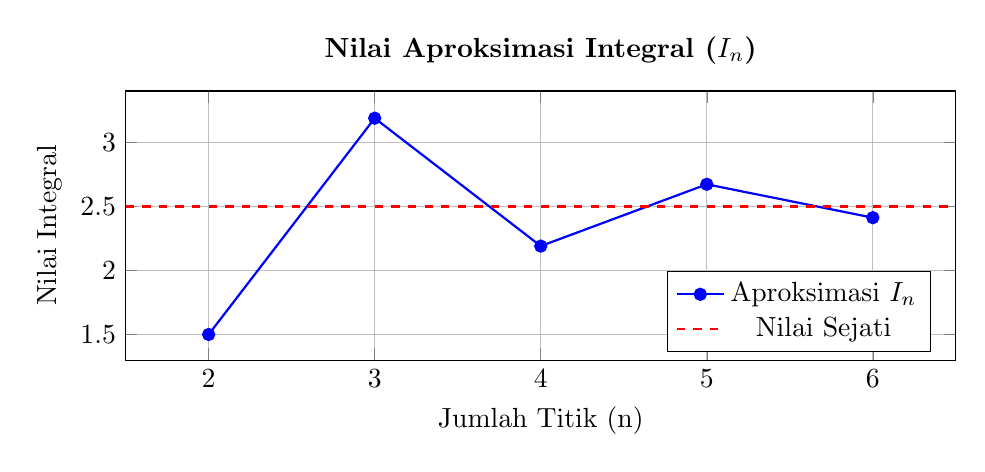
\begin{tikzpicture}
    \begin{axis}[
        title={\textbf{Nilai Aproksimasi Integral ($I_n$)}},
        xlabel={Jumlah Titik (n)},
        ylabel={Nilai Integral},
        xmin=1.5, xmax=6.5,
        ymin=1.3, ymax=3.4,
        xtick={2,3,4,5,6},
        grid=major,
        legend pos=south east,
        width=\columnwidth, % <-- ini yang penting
        height=5cm,
    ]
        
    % Plot 1: Data aproksimasi I_n
    \addplot[
        color=blue,
        mark=*,          % Beri tanda (*) pada setiap titik data
        thick,           % Tebalkan garis plot
    ] coordinates {
        (2, 1.50000)
        (3, 3.18750)
        (4, 2.18978)
        (5, 2.67170)
        (6, 2.41136)
    };
    \addlegendentry{Aproksimasi \(I_n\)} % Label untuk plot pertama
    
    % Plot 2: Garis horizontal untuk Nilai Sejati
    \addplot[
        color=red,
        dashed,          % Gaya garis putus-putus
        thick,
        domain=1.5:6.5,  % Rentang gambar garis dari xmin hingga xmax
    ] {2.4980915}; % Nilai y konstan (nilai sejati)
    \addlegendentry{Nilai Sejati} % Label untuk plot kedua
        
    \end{axis}
\end{tikzpicture}
\caption{Grafik perbandingan nilai aproksimasi integral ($I_n$) terhadap nilai target untuk jumlah titik (n) yang berbeda.}
\label{fig:grafik_aproksimasi_integral}
\end{figure}

Pada visualisasi grafik diatas, terlihat bahwa nilai aproksimasi integral ($I_n$) untuk setiap formula Gauss-Legendre (dari 2 hingga 6 titik) berfluktuasi, namun secara umum mendekati nilai target yang ditandai dengan garis horizontal merah. Formula 2-titik menunjukan nilai paling jauh dari nilai sejati, yaitu sekitar 1.5, sedangkan formula 6-titik memberikan hasil yang paling mendekati nilai sejati, yaitu sekitar 2.41136. Hal ini menunjukkan bahwa semakin banyak titik yang digunakan dalam formula Gauss-Legendre, semakin akurat aproksimasi integral yang dihasilkan.

\begin{figure}[htbp]
\centering
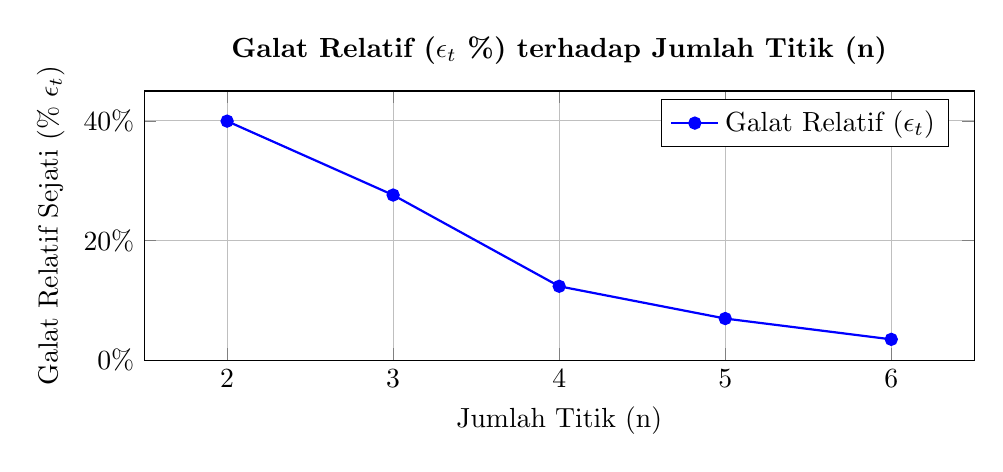
\begin{tikzpicture}
    \begin{axis}[
        title={\textbf{Galat Relatif ($\epsilon_t$ \%) terhadap Jumlah Titik (n)}},
        xlabel={Jumlah Titik (n)},
        ylabel={Galat Relatif Sejati (\% \(\epsilon_t\))},
        xmin=1.5, xmax=6.5,  % Memberi sedikit ruang di tepi
        ymin=0, ymax=45,     % Mulai sumbu y dari 0
        xtick={2,3,4,5,6},   % Tentukan titik-titik pada sumbu x
        yticklabel={\pgfmathprintnumber{\tick}\%}, % Tambahkan simbol % pada sumbu y
        grid=major,          % Tambahkan grid utama
        legend pos=north east, % Posisi legenda
        width=\columnwidth, % Lebar grafik agar pas di kolom
        height=5cm,
    ]
        
    % Data plot diambil dari hasil output program C
    \addplot[
        color=blue,
        mark=*,          % Beri tanda (*) pada setiap titik data
        thick,           % Tebalkan garis plot
    ] coordinates {
        (2, 39.95416)
        (3, 27.59740)
        (4, 12.34184)
        (5, 6.94956)
        (6, 3.47205)
    };
    
    % Menambahkan entri untuk legenda
    \addlegendentry{Galat Relatif (\(\epsilon_t\))}
        
    \end{axis}
\end{tikzpicture}
\caption{Grafik visualisasi penurunan galat relatif sejati seiring dengan bertambahnya jumlah titik (n) pada metode Gauss-Legendre.}
\label{fig:grafik_galat_konvergensi}
\end{figure}

Dari hasil yang divisualisasikan pada grafik diatas, terlihat jelas bahwa akurasi metode Gauss-Legendre meningkat secara dramatis dengan penambahan jumlah titik. Formula 2-titik memberikan hasil yang cukup tinggi sebesar 39.954\%. Namun, saat formula 6-titik digunakan, galatnya turun drastis hingga sebesar 3.472\%.

\section{KESIMPULAN}
Perhitungan membuktikan bawa formula Gauss-Legendre sangat efisien dalam mengaproksimasi integral dari fungsi kontinu seperti $\int_{-3}^{3} \frac{1}{1+x^2} dx$. Dengan hanya 6 kali evaluasi fungsi, metode ini menghasilkan aproksimasi yang sangat dekat dengan nilai target. Galat relatif sejati menurun dari 39.95\% untuk formula 2-titik menjadi hanya 3.472\% untuk formula 6-titik. Metode ini secara optimal memilih titik evaluasi untuk menangkap "perilaku" fungsi di seluruh interval sehingga menghasilkan konvergensi yang cepat menuju solusi yang benar.

\section{LINK GITHUB}
https://github.com/BonifasiusRaditya/FinproKomputasiNumerik.git

\section{LINK YOUTUBE}
\url{https://youtu.be/ITIelyhhZOo} \\

\begin{thebibliography}{00}
\bibitem{ref1} F. M. White, \textit{Fluid Mechanics}, 8th ed. New York: McGraw-Hill Education, 2016.
\bibitem{ref2} S. C. Chapra and R. P. Canale, \textit{Numerical Methods for Engineers}, 7th ed. New York: McGraw-Hill Education, 2015.
\bibitem{ref3} J. D. Anderson, \textit{Computational Fluid Dynamics: The Basics with Applications}, 2nd ed. New York: McGraw-Hill Education, 1995.
\bibitem{ref4} E. Kreyszig, \textit{Advanced Engineering Mathematics}, 10th ed. New York: Wiley, 2011.
\end{thebibliography}
\vspace{12pt}

\end{document}